
\section{Etape 4 : apprentissage des préférences}

\subsection{Modélisation du score}

On modélise le score sur les 3 dimenssions de la facçon suivante (sous la forme UTA):

Le score est la somme des dimensions pondéré par un poids, 
le poid est une fonction linéaire par morceau sur chaque dimension, 
monotone, croissante et continue. qui vaut 0 pour la valeur minimale 
et 1 pour la valeur maximale. x etant un vecteur de taille 3, 
le score est donc donné par:

\begin{equation}
    score(x) = \sum_{i=1}^{3} \omega_i(x_i) \times x_i
\end{equation}

avec en prenant $\omega_i^k$ la valeur de $\omega_i$ en $x_i^k$:

\begin{equation}
    \omega_i(x_i) = \omega_i^k + (x_i - x_i^k) \times \frac{\omega_i^{k+1} - 
    \omega_i^k}{x_i^{k+1} - x_i^k} \text{   avec   } x_i^k \leq x_i \leq x_i^{k+1}
\end{equation}

et :

\begin{equation}
    x_i^k = min_i + k \frac{max_i - min_i}{L_i} 
\end{equation}

Les paramêtres à déterminer sont donc les $(w_i^k)_{i=1,2,3;\ k \in |[0,L_i]|}$


Les valeurs minimales et maximales étant définis arbitraiement suivant les classements, 
on extrapole les fonction $\omega_i$ pour les valeurs inférieures et supérieures à $x_i^0$ 
et $x_i^{L_i}$ par les valeurs constante $\omega_i^0$ et $\omega_i^{L_i}$.

\subsection{Optimisation du score}

à partir du classement effectué par l'agent, on approxime le score pour chaque SR 
classé de la façon suivante (on dispose de n SR classé avec leur scores):

\begin{equation}
    H(x^t) =  score(x^t) + \epsilon^t
\end{equation}

avec $\epsilon^t$ une variable du problème d'optimisation.

On fixe un seuil $\delta = 1e^{-2}$ (pour avoir un ranking ) et on ajoute les contraintes suivante:

\begin{equation}
    \forall t \in [1,n-1],\ H(x^t) \leq H(x^{t+1})) - \delta
\end{equation}

et on minimise la somme des $\epsilon^t$. la fonction objectif est donc:

\begin{equation}
    \min( \sum_{t=1}^{n} \epsilon^t )
\end{equation}

\subsection{Résultats}

On a donc utilisé la librairie gurobi pour résoudre ce problème d'optimisation.

On a utilisé les données de l'agent pour déterminer les paramètres $\omega_i^k$. On 
a choisi de prendre $L_i = 5$ pour chaque dimension. On a donc 30 paramètres à déterminer. 
Les résultats sont données dans la figure \ref{fig:omega}.

\begin{figure}[H]
    \centering
    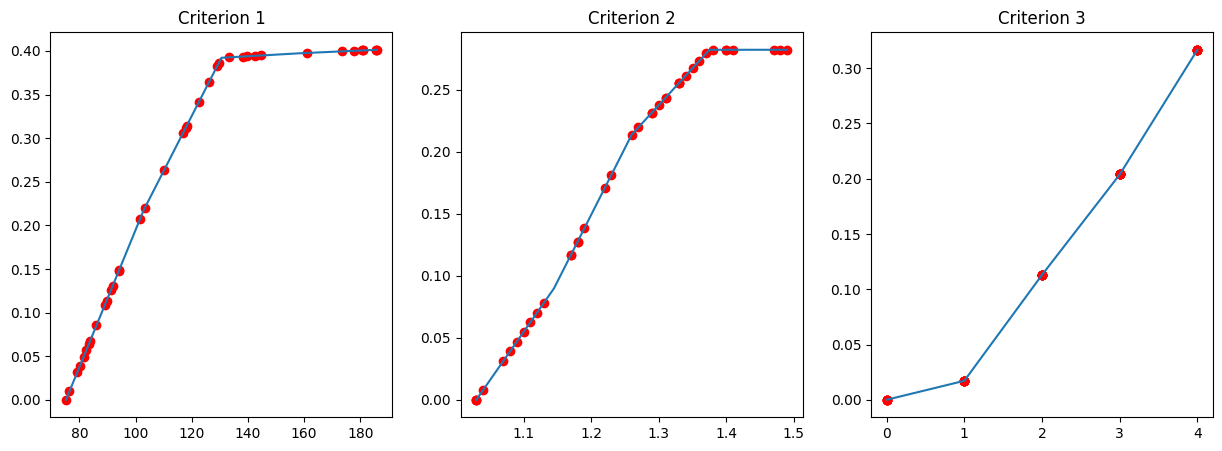
\includegraphics[width=0.8\textwidth]{Images/step_4/resultats_omega.png}
    \caption{Valeurs des poids $\omega_i^k$ trouvés par optimisation}
    \label{fig:omega}
\end{figure}

On a ensuite utilisé ces paramètres pour déterminer le classement des SR en
comparant le score des solutions non-dominés. Les résultats sont donnés dans 
le tableau \ref{tab:valeurs}.

\begin{table}[H]
    \centering
    \begin{tabular}{|c||c||c|c|c|}
        \hline
        Index & Score & Distance & Max worload & Changed offices \\
        \hline
        1 & 0.314 & 114.94 & 1.03 & 1 \\
        \hline
        2 & 0.322 & 112.92 & 1.06 & 1 \\
        \hline
        3 & 0.331 & 108.81 & 1.1 & 1 \\
        \hline
        4 & 0.333 & 112.62 & 1.08 & 1 \\
        \hline
        5 & 0.387 & 111.79 & 1.01 & 2 \\
        \hline
    \end{tabular}
    \caption{Les 5 premières solutions pour l'organisation des SR.}
    \label{tab:valeurs}
\end{table}
